\documentclass[fleqn]{article}
\oddsidemargin 0.0in
\textwidth 6.0in
\thispagestyle{empty}
\usepackage{import}
\usepackage{amsmath}
\usepackage{graphicx}
\usepackage{flexisym}
\usepackage{calligra}
\usepackage{amssymb}
\usepackage{bigints} 
\usepackage[english]{babel}
\usepackage[utf8x]{inputenc}
\usepackage{float}
\usepackage[colorinlistoftodos]{todonotes}


\DeclareMathAlphabet{\mathcalligra}{T1}{calligra}{m}{n}
\DeclareFontShape{T1}{calligra}{m}{n}{<->s*[2.2]callig15}{}
\newcommand{\scriptr}{\mathcalligra{r}\,}
\newcommand{\boldscriptr}{\pmb{\mathcalligra{r}}\,}

\definecolor{hwColor}{HTML}{442020}

\begin{document}

  \begin{titlepage}

    \newcommand{\HRule}{\rule{\linewidth}{0.5mm}}

    \center

    \begin{center}
      
\includegraphics[height=11cm, width=11cm]{asu.png}
    \end{center}

    \vline

    \textsc{\LARGE Classical Parts/Field/Matter III}\\[1.5cm]

    \HRule \\[0.5cm]
    { \huge \bfseries Homework 8}\\[0.4cm] 
    \HRule \\[1.0cm]

    \textbf{Behnam Amiri}

    \bigbreak

    \textbf{Prof: Samuel Teitelbaum}

    \bigbreak

    \textbf{{\large \today}\\[2cm]}

    \vfill

  \end{titlepage}

  \begin{enumerate}
    \item \textbf{10.15 (60 points)} A particle of charge $q$ moves in a circle of radius $a$ at constant
    angular velocity $\omega$. (Assume that the circle lies in the x y plane, centered at the
    origin, and at time $t = 0$ the charge is at $(a, 0)$, on the positive x axis.) Find the
    Liénard-Wiechert potentials for points on the $z$ axis.

        \textcolor{hwColor}{
          \\
          The Liénard-Wiechert potentials describe the classical electromagnetic effect of a moving 
          electric point charge in terms of a vector potential and a scalar potential in the Lorenz gauge.
          We learned that the \textbf{Liénard-Wiechert potentials} for a moving point charge are:
          \\
          \\
          $
            \begin{cases}
              V(\mathbf{r},t)=\dfrac{1}{4 \pi \epsilon_0} \dfrac{qc}{\bigg( \scriptr c- \mathbf{\scriptr}.\mathbf{v} \bigg)}
              \\
              \\
              A(\mathbf{r},t)=\dfrac{\mu_0}{4 \pi} \dfrac{qc \mathbf{v}}{\bigg( \scriptr c- \mathbf{\scriptr}.\mathbf{v} \bigg)}
              =\dfrac{\mathbf{v}}{c^2} V(\mathbf{r},t)
            \end{cases}
            \\
            \\
          $
          According to the setup of this problem, we can simulate the charge move with a sinusoidal function as:
          \\
          \\
          $
            r(t)=a \left[
              cos(\omega t) ~ \hat{x}+sin(\omega t) ~ \hat{y}
            \right]
          $
          \\
          \\
          \text{The above equation satifies the following condition which is what we wanted:}
          \\
          \\
          $
            \boxed{t=0 \longrightarrow r(0)=r(t)=a \left[cos(\omega \times 0) ~ \hat{x}+sin(\omega \times 0) ~ \hat{y}\right]=a}
            \\
            \\
            \\
            \text{The velocity of the particle is:}
            \\
            \\
            \dfrac{\partial r}{\partial t}
            =\dfrac{\partial}{\partial t} \bigg( a \left[cos(\omega t) ~ \hat{x}+sin(\omega t) ~ \hat{y}\right] \bigg)
            \\
            \\
            \dfrac{\partial r}{\partial t}=a \dfrac{\partial}{\partial t} \bigg( \left[cos(\omega t) ~ \hat{x}+sin(\omega t) ~ \hat{y}\right] \bigg)
            =a \bigg( -\omega ~ sin(\omega t) ~ \hat{x}+\omega ~ cos(\omega t) ~ \hat{y} \bigg)
            \\
            \\
            \\
            \therefore ~~~ \boxed{
              v(t)=a \omega \bigg( -sin(\omega t) ~ \hat{x}+cos(\omega t) ~ \hat{y} \bigg)
            } ~~~~ \checkmark
            \\
            \\
            \\
            \text{From page 9, chapter 1, we learned that definition of } \scriptr \text{ as:}
            \\
            \\
            \begin{cases}
              \scriptr \equiv r- r^' ~~~~ \text{Field point minus source point}
              \\
              \\
              \scriptr=\bigg( x-x^' \bigg) ~ \hat{x}+\bigg( y-y^' \bigg) ~ \hat{y}+\bigg( z-z^' \bigg) ~ \hat{z}
            \end{cases}
            \\
            \\
            \\
          $
          Consider a point at a distance $z$ from the center along the z-axis, therefore field point minus 
          source point gives us.
          \\
          \\
          $ 
            \scriptr=r-r^'=z ~ \hat{z}- \bigg( a \left[
              cos(\omega t) ~ \hat{x}+sin(\omega t) ~ \hat{y}
            \right] \bigg) 
            \\
            \\
            \\
            \therefore ~~~ \boxed{
              \scriptr=-a ~ cos(\omega t) ~ \hat{x}-a ~ sin(\omega t) ~ \hat{y}+z ~ \hat{z}
            } ~~~~ \checkmark
            \\
            \\
            \\
            \scriptr^2=\left[
              -a ~ cos(\omega t) ~ \hat{x}-a ~ sin(\omega t) ~ \hat{y}+z ~ \hat{z}
            \right]^2
            =\left[ -a ~ cos(\omega t) ~ \hat{x}-a ~ sin(\omega t) ~ \hat{y}+z ~ \hat{z} \right] 
            \left[ -a ~ cos(\omega t) ~ \hat{x}-a ~ sin(\omega t) ~ \hat{y}+z ~ \hat{z} \right]
            \\
            \\
            \\
            \scriptr^2=a^2 ~ cos^2(\omega t) ~ \hat{x}.\hat{x}
            +a^2 ~ cos(\omega t) sin(\omega t) ~ \hat{x}.\hat{y}
            -az ~ cos(\omega t) ~ \hat{x}.\hat{z}
            +a^2 ~ sin(\omega t) cos(\omega t) ~ \hat{y}.\hat{x}
            +a^2 ~ sin^2(\omega t) ~ \hat{y}.\hat{y}
            -az ~ sin(\omega t) ~ \hat{y}.\hat{z}
            -az ~ cos(\omega t) ~ \hat{z}.\hat{x}
            -az ~ sin(\omega t) ~ \hat{z}.\hat{y}
            +z^2 ~ \hat{z}.\hat{z}
            \\
            \\
            \\
            \scriptr^2=a^2 ~ cos^2(\omega t)+a^2 ~ sin^2(\omega t)+z^2
            =a^2 \left[cos^2(\omega t)+sin^2(\omega t)\right]+z^2
            \\
            \\
            \\
            \therefore ~~~ \boxed{
              \scriptr^2=a^2+z^2 
            } ~~~~ \checkmark
            \\
            \\
            \\
            \hat{\scriptr}=\dfrac{\scriptr}{\scriptr}=\dfrac{
              -a ~ cos(\omega t) ~ \hat{x}-a ~ sin(\omega t) ~ \hat{y}+z ~ \hat{z}
            }{
              \sqrt{a^2+z^2}
            }
            \\
            \\
            \\
            \hat{\scriptr}.v=\bigg( 
              \dfrac{
                -a ~ cos(\omega t) ~ \hat{x}-a ~ sin(\omega t) ~ \hat{y}+z ~ \hat{z}
              }{
                \sqrt{a^2+z^2}
              }  
            \bigg).\bigg( 
              a \omega \bigg( -sin(\omega t) ~ \hat{x}+cos(\omega t) ~ \hat{y} \bigg)
            \bigg)=a^2 \omega ~ sin(\omega t) cos(\omega t)-a^2 \omega ~ sin(\omega t) cos(\omega t)
            \\
            \\
            \\
            \therefore ~~~ \boxed{
              \hat{\scriptr}.v=0
            } ~~~~ \checkmark
            \\
            \\
            \\
            \text{From page 455 of the textbook we know } t_r=t \pm \dfrac{\scriptr}{c} \text{, hence: (we want the minus sign)}
            \\
            \\
            t_r=t - \dfrac{\scriptr}{c}=\dfrac{ct-\scriptr}{c} \Longrightarrow \scriptr=c \bigg( t-t_r \bigg)
            \Longrightarrow \hat{\scriptr}=\dfrac{r-v t_r}{c \bigg( t-t_r \bigg)}
            \\
            \\
            \\
            \text{Knowing that } \hat{\scriptr}.v=0 \Longrightarrow 1-\dfrac{\hat{\scriptr}.v}{c}=1
            \\
            \\
            \\
            \therefore ~~~ \boxed{
              \begin{cases}
                V(\mathbf{r},t)=V(z,t)=\dfrac{1}{4 \pi \epsilon_0} \dfrac{q}{\sqrt{a^2+z^2}}
                \\
                \\
                A(\mathbf{r},t)=A(z,t)
                =\dfrac{q}{4 \pi \epsilon_0 c^2} \dfrac{
                  a \omega \bigg( -sin(\omega t_r) ~ \hat{x}+cos(\omega t_r) ~ \hat{y} \bigg)
                  }{
                    \sqrt{a^2+z^2}
                  }
              \end{cases}
            } ~~~~ \checkmark
            \\
            \\
          $
        }

    \item \textbf{10.16 (20 points)} Show that the scalar potential of a point charge moving with constant 
    velocity (Eq. $10.49$) can be written more simply as
    $$
      V(r,t)=\dfrac{1}{4 \pi \epsilon_0} \dfrac{q}{R\sqrt{1-v^2 ~ sin^2 ~ \theta/c^2}},
    $$
    where $R \equiv r-vt$ is the vector from the present $(!)$ position of the particle to the
    field point $r$, and $\theta$ is the angle between $R$ and $v$ (Fig. 10.9). Note that 
    for nonrelativistic velocities $(v^2 << c^2)$,
    $$
      V(r,t) \approx \dfrac{1}{4 \pi \epsilon_0} \dfrac{q}{R}
    $$
    \emph{Note the denominator looks a lot like the lorentz factor.}
    \begin{center}
      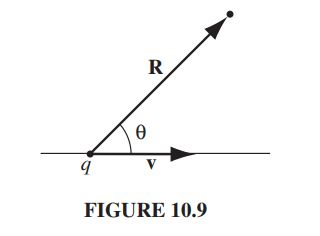
\includegraphics[height=5cm, width=7cm]{1.JPG}
    \end{center}

        % \textcolor{hwColor}{
        %   \\
        % }

    \item \textbf{10.25 (20 points)} Figure $2.35$ summarizes the laws of electrostatics in a "triangle
    diagram" relating the source $(\rho)$, the field $(E)$, and the potential $(V)$. Figure $5.48$
    does the same for magnetostatics, where the source is $J$, the field is $B$, and the
    potential is A. Construct the analogous diagram for electrodynamics, with sources
    $\rho$ and $J$ (constrained by the continuity equation), fields $E$ and $B$, and potentials $V$
    and $A$ (constrained by the Lorenz gauge condition). Do not include formulas for $V$
    and $A$ in terms of $E$ and $B$.
    \begin{center}
      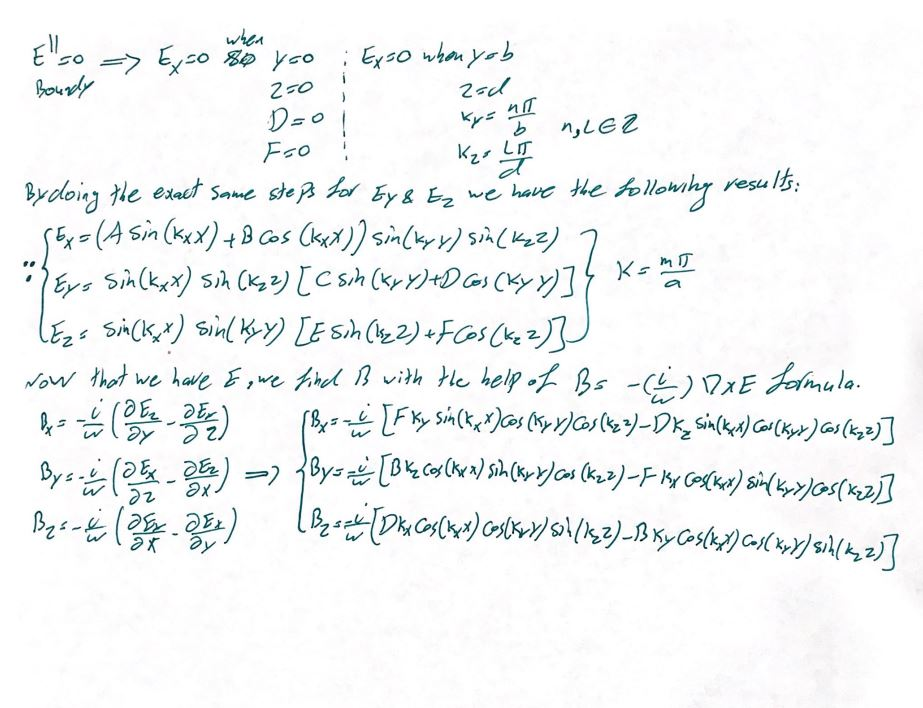
\includegraphics[height=7cm, width=7cm]{2.JPG}
    \end{center}

        % \textcolor{hwColor}{
        %   \\
        % }
    
  \end{enumerate}

\end{document}
